
Our goal is to build a collaborative drawing agent, through communication in language. In the Sketch-RNN work, the model can complete a partial sketch done by the users. In our case, we want to augment this collaborative creative process with language. A user can not only draw part of the sketch but also specify to the robot what kind of sketches they want to create: an angel with cloud-shaped wings or a face with angry-looking eyes. 
Learning sketch representations comes with its own challenges due to its abstractness, but how similar shapes are used in different context and how similar language is used in different context also makes learning sketch representation interesting, especially when most of the state of the art vision-language work focuses on RGB image data, we want to know how well SOTA methods generalize to the sketch domain. To advance towards a collaborative drawing agent, we choose sketch for its abstractness. 
The abstract nature of sketches brings both challenges and simplication of the problem. Challenges are about pretrained large vision-language models like CLIP are trained on RGB image data, simplification is about the fact that things like paintings with brushes bring in more manipulative challenges, so if we do want to study how language interacts with users or users interact with robots, it comes with its own research questions. Therefore, there are a couple of disparate directions that we can take this project. Simplication: it reduces the manipulation challenges with handling different art tools and techniques related to painting.   
\begin{enumerate}
    \item How well does current vision-language joint embeddings capture the abstract sketch representation? We are interested in this question because (1) CLIP is not trained with sketches and is trained mostly with RGB images; (2) humans are able to generalize concepts like small, large  
\end{enumerate}

We utilize CLIP to gain more insights into our dataset, beyond simple counting statistics. Given the nature of our dataset: a large variety of words but most words have very few occurrences, small number of images, text descriptions are contrastively collected by juxtaposing two images with opposite features, similar descriptions used for different purpose in different context. How does CLIP respond to this dataset, how well does CLIP embeddings align with our intuitions about these tasks? Specifically, for transferring the same word to be used in different context, or usage of words that are not the common meaning of words, how well can CLIP handle them, since it is trained on millions of images? Even though CLIP is not on the sketch domain, CLIP was trained on a large number of images on the internet, and there are GAN methods that have taken advantag eof CLIP embeddings to guide image generation: ClipDraw, StylCLIP, CLIP-NADA.      

\section{Task Definition} \label{modeling.task.def}
Given two sketches $(s_1,s_2)$ and their part annotations $(t_1,t_2)$, determine which sketch $t_1$ should pair with, similarly for $t_2$. 
During data collection, we implicitly juxtapose two sketches, chosen to be as distinct as possible using some heuristic, either from different clusters or whose cosine distance is large, so the process of annotating the two dissimilar sketches is like the annotators are choosing the pair up one annotation with another. Implicitly, the annotators is pairing $s_1$ with $t_1$ and $s_2$ with $t_2$, so we would regard the ground truth pairing to be $(s_1,t_1)$ and $(s_2,t_2)$. We want to see how CLIP does on this task, if it is the annotator for the task, would it be able to generate the same pairing. Define cosine similarity to be.  



Given $(s_1,s_2)$, we use CLIP image encoder (zero-shot/fine-tuned) $f_v$ to extract visual features for the two sketches,  $f_v(s_1) \in {R}^{512}$, and $f_v(s_2) \in {R}^{512}$. We then use the zero-shot/fine-tuned CLIP text encoder to extract the text features for the part descriptions, namely we fill in the template $t = \texttt{[ADJ] [PART NAME]}$, where $\texttt{[ADJ]}$ is filled with the adjective phrases annotations, and $\texttt{[PART NAME]}$ is the name of the part in the sketches. For angels, $\texttt{[PART NAME]}$ is one of \textit{halo}, \textit{eyes}, \textit{nose}, \textit{mouth}, \textit{body}, \textit{outline of face}, \textit{wings}; for face, $\texttt{[PART NAME]}$ is one of \textit{eyes}, \textit{nose}, \textit{mouth}, \textit{hair}, \textit{outline of face}. After filling in the above template, we obtain the part annotations for the two sketches $t_1,t_2$.  
We obtain embeddings for the part annotations by encoding them through CLIP text encoder $f_t$: $f_t(t_1) \in {R}^{512}$, and $f_t(t_2) \in {R}^{512}$. We then calculate cosine similarity between all four pairs of $(f_v(s_i), f_t(t_j))$, $i,j \in [2]$, where consine similarity between two vectors $u,v$ is defined as $S_c(u,v) = \dfrac{u \cdot v}{\|u\| \|v\|}$. 
\begin{equation}
    \begin{split}
        I_1, I_2 \\
        T_1, T_2 \\
        S_c(I_i,T_j) & = \dfrac{I_i \cdot T_j}{\|I_i\| \|T_j\|} \\
        S_c(u,v) & = \dfrac{u \cdot v}{\|u\| \|v\|} \\
        f(j) & = \max_{i} S_c(f_v(s_i), f_t(t_j)) \hspace{2em} i \in [2]
    \end{split}
\end{equation}
Therefore, given that our entire pipeline is $f$, $f(j) \in [2]$ output which of the two sketches $t_j$ will be paired with, and $$f(j) = \max_{i} S_c(f_v(s_i), f_t(t_j)) \hspace{2em} i \in [2]$$.    

\section{Metric}

Given $n$ pairs of two sketches and two part annotations, the same pairs that were provided by the annotators, we calculate an accuracy-like metric:
$$ acc = \frac{\sum_{k=1}^{n} \sum_{j=1}^2 \mathbbm{1}{(f(j) = j)}}{2n} $$

\section{Method}

We utilized the \texttt{Python} \texttt{clip} package and load their pre-trained CLIP model, specifically the \texttt{ViT-B/32} variant, which uses the Vision Transformer \citep{visiontransformer} as the image encoder; \texttt{B} stands for \textit{Base} model, and \texttt{32} stands for $32 \times 32$ input patch size. CLIP has two main parts: a text encoder and an image encoder, and both are transformer based. We will divide this section into explaining the two encoders. When introducing the text encoder, we will briefly introduce the encoder-decoder recurrent neural networks (RNN), which are the state-of-the-art method predating transformers, and their shortcomings in terms of inefficiency handling long sequences; we then introduce the self-attention mechanism and transformer models. In this way, we have better understanding of the advantages of modeling large corpus with transformer models. 
Transformers are first tested in natural language processing tasks and then adapted to vision tasks,

\subsection{Text Encoder}

\paragraph{Before Transformer: Recurent Neural Networks}
Traditionally, recurrent neural network's (RNN), such as long short-term memory (LSTM) and gated reccurent unit (GRU) recurrent network, are used in language modeling.
The sequential nature of RNN's precluded them efficient parallelization and resulted in difficulty modeling longer sequences \citep{attentionAllYouNeed}. 
\citet{encoderDecoderRNN} and \citet{encoderDecoderRNN2} introduced the framework of using neural networks, specifically 
RNNs, for language modeling. The framework works as follows:  
if given a sequence of $T$ words $\mathbf{x} =  (x_1,x_2,\dots, x_{T})$, an RNN encoder compute a sequence of hidden states $h_t = f(h_{t-1}, x_t)$, where $h_{t-1}$ is the previous hidden state, and $x_t$ is the current input. It then compresses all the $T$ hidden states into one context vector $c = q(\{h_1,\dots,h_T\})$, where $q$ is some nonlinear function. Therefore, summarizing the input sequence into a representation is carried out in a sequential manner.  
The decoding process is sequential too: $c$ and outputs from previous time steps are used to generate the output of the current step $t$, $y_t = g(c, h_t^{'}, y_1,\dots,y_{t-1})$, where $g$ is some nonlinear transformation, and $h_t^{'}$ is the hidden state in the decoder \citep{encoderDecoderRNN,encoderDecoderRNN2}.
In this way, the encoder-decoder RNN architecture models the output sentence sequence $\mathbf{y}$ as the product of conditionals of each time step: $\mathbf{y} = \prod_{t=1}^T p(y_t | c,y_1,\dots,y_{t-1})$.  
During both encoding and decoding, the RNN architecture constrains the modeling to be sequential \citep{attentionRNN}. Moreover, the sequential nature of RNN limits the ability to model long-range dependencies among parts of the sentences, which is crucial in many cases. 

\paragraph{RNN with Attention}
The attention mechanism, the foudational building block of transformer, has been used with RNN's before. 
Introduced in \citet{attentionRNN}, attention is used to alleviate the problem of compressing all information extracted from the input sequence in one fixed context vector $c$ to compute the output at every time step. In the aforementioned 
$y_t = g(c, h_t^{'}, y_1,\dots,y_{t-1})$, \citet{attentionRNN} altered the fixed $c$ into an hidden state dependent $c_t$, and it is computed as the weighted sum of the encoder hidden states $h_j$: $c_t = \sum_{j=1}^{T} \alpha_{tj} h_j$. The weight $\alpha_{tj}$ represents how well $h_j$, the hidden state corresponding to the $j$-th word in the input, align with the decoder hidden state $h_{t-1}^{'}$ just before the current decoding step $t$. In this way, $c_t$ summarize the input in an output-dependent way, making inputs that associate with $y_t$ more closely contribute more to modeling $ p(y_t | c_t,y_1,\dots,y_{t-1})$.   

\paragraph{Transformer: Attention is All You Need}
\begin{figure*}[!htb]
\begin{subfigure}{0.5\textwidth}
    \centering
    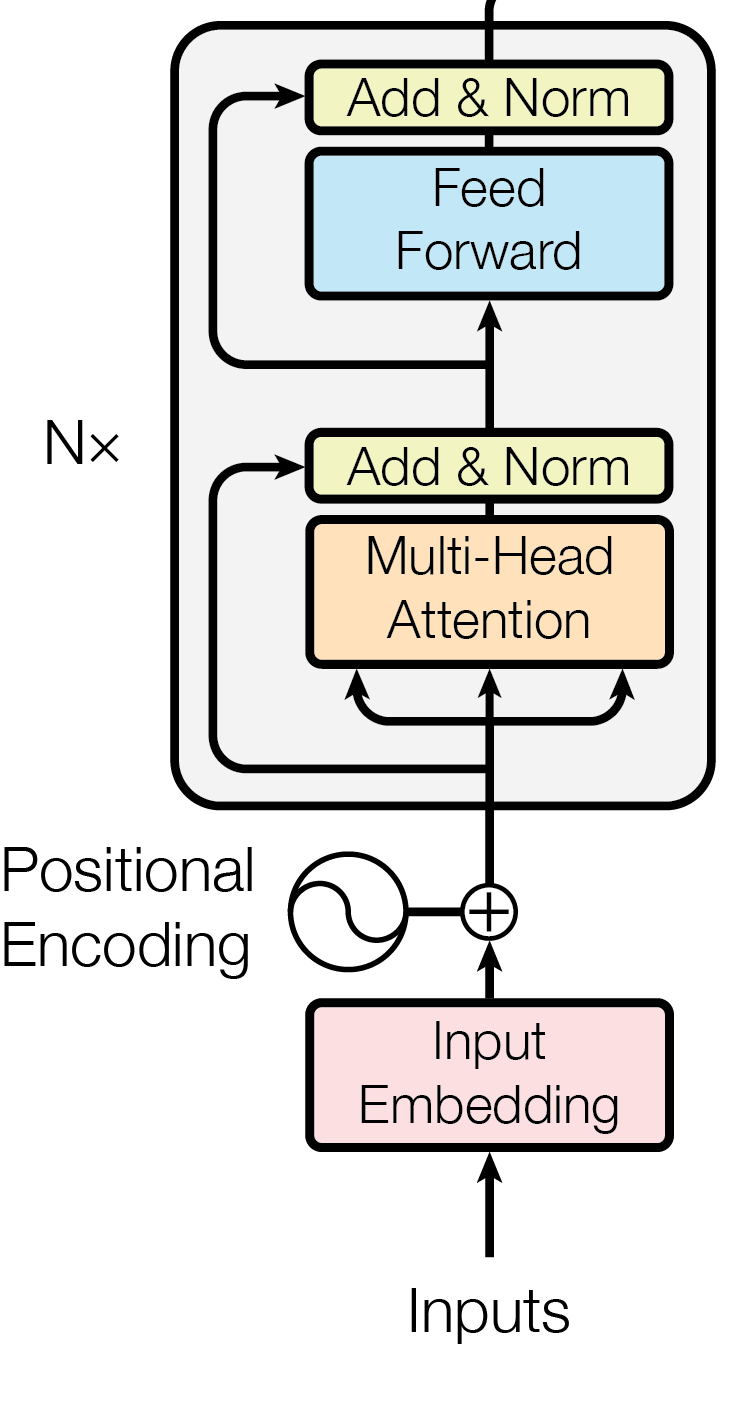
\includegraphics[width=0.5\linewidth]{modeling/transformer.png}  
    \caption{Encoder architecture used in original Transformer paper \citep{attentionAllYouNeed}.}
    \label{modeling.transformer.origEncoder}
\end{subfigure}
\begin{subfigure}{0.5\textwidth}
    \centering
    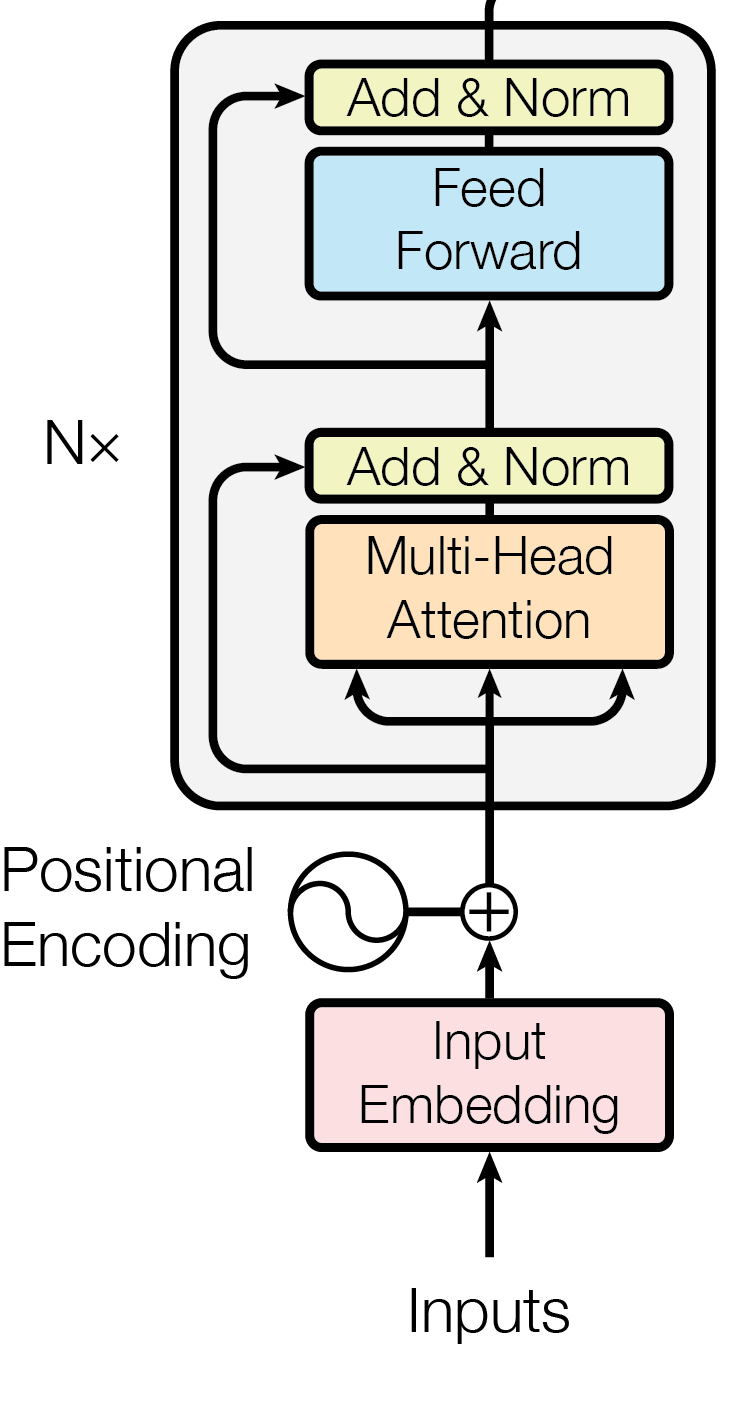
\includegraphics[width=0.5\linewidth]{modeling/transformer.png}   
    \caption{Encoder architecture of CLIP \citep{CLIPpaper}.}
    \label{modeling.attention.clipEncoder}
\end{subfigure}
\caption{Transformer architecture.}
\label{modeling.transformer}
\end{figure*}

The text encoder of CLIP is based on the transformer architecture introduced in \citet{attentionAllYouNeed}, and transformer relies only on the self-attention mechanism to compute a representation for the input sequence. In this way, it alleviates the computation efficiency and long-range dependencies problems witnessed in recurrent layers.  
Figure \ref{modeling.transformer.origEncoder} and \ref{modeling.attention} are the same figures used in \cite{attentionAllYouNeed} to illustrate the transformer architecture. In Figure \ref{modeling.transformer.origEncoder}, \cite{attentionAllYouNeed} gives an overview of the encoder architecture; tokenized texts go through an embedding layer, and the input embeddings are summed with learned position embeddings that inject information on order of the sequence. 
% and incorporated modification suggested in \citet{Radford2019LanguageMA}
The input is computed using Byte Pair Encoding (BPE) with a $49,152$ vocabulary. As explained in \cite{Radford2019LanguageMA}, BPE, a sub-word tokenization scheme, strikes a good balance between word-level and character-level word embeddings, since one works well with common words and the other with rare sequences.
The input is then passed through stacked layers multi-head attention (MHA) mechanism followed by point-wise feed-forward networks (FFN). 
In the version of CLIP that we use, the text encoder is a 12-layer transformer, and the model dimenison is $512$, $d_{model} = 512$, meaning that output of the initial embedding layers, MHA, FFN all have dimension $512$.  
Compare to the formulation $LayerNorm(x + Sublayer(x))$ used in \cite{attentionAllYouNeed} (Figure \ref{modeling.transformer.origEncoder}), the CLIP text encoder uses $x + Sublayer(LayerNorm(x))$ (Figure \ref{modeling.attention.clipEncoder}), where $Sublayer$ refers to either MHA or FFN, so each layer still contains residual connection and layer normalization, but the order is switched. 


\begin{figure*}[!htb]
\begin{subfigure}{0.5\textwidth}
    \centering
    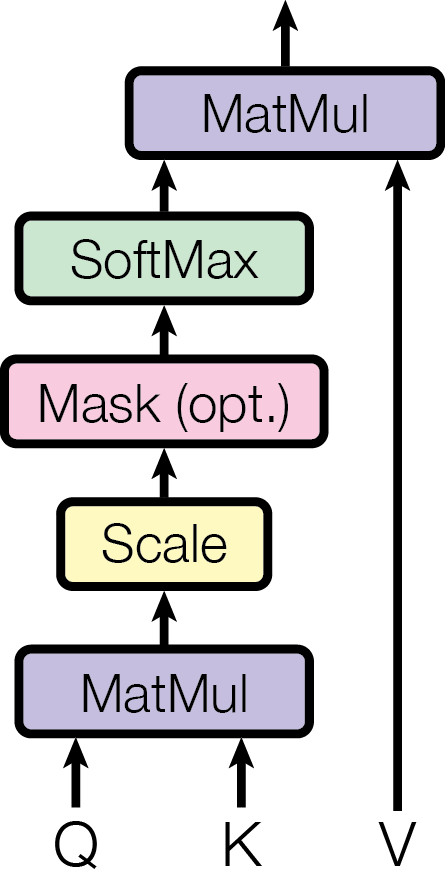
\includegraphics[width=.3\linewidth]{modeling/selfAttention.png}  
    \caption{.}
    \label{modeling.attention.dot}
\end{subfigure}
\begin{subfigure}{0.5\textwidth}
    \centering
    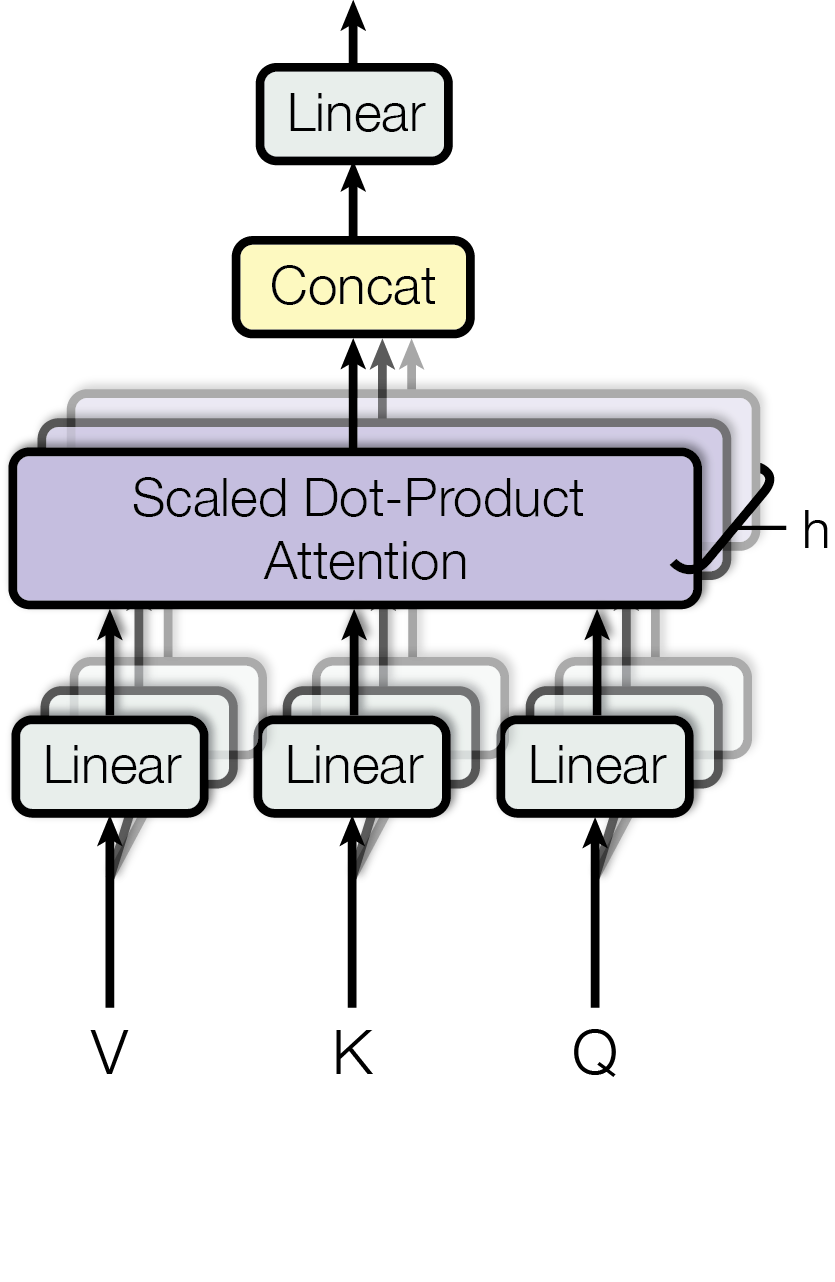
\includegraphics[width=.5\linewidth]{modeling/multiHeadAttention.png}  
    \caption{.}
    \label{modeling.attention.multihead}
\end{subfigure}
\caption{Screenshots of counterexamples used in first version of the requirements in Version 1.}
\label{modeling.attention}
\end{figure*}

As illustrated in Figure \ref{modeling.attention.multihead}, given query, key, value matricies $Q,K,V$ (in our case, all three matrices equal to the input text embeddings), transformer uses different linear projections to create multi-head attention, and \citet{attentionAllYouNeed} explains the benefit of multi-head attention as allowing the model to attend simultaneously to multiple representation subspaces of the input.      

\begin{equation} \label{mha}
\begin{split}
    MultiHead(Q,K,V) & = Concat({head}_1,\dots,{head}_h)W^O \\
    {head}_i & = Attention(QW_i^{Q}, KW_i^{K}, VW_i^{V}) \\
    Attention(Q,K,V) & = softmax(\dfrac{QK^T}{\sqrt{d_k}})V 
\end{split}
\end{equation}

$\text{ViT-B}/32$ uses a version with $h = 8$ attention heads, so $W_i^{Q}, W_i^{K} \in \mathbb{R}^{d_{model} \times d_k}$ and $W_i^{V} \in \mathbb{R}^{d_{model} \times d_v}$, where $d_k = d_v = \dfrac{d_{model}}{h} = \frac{512}{8} = 64$. 
At the end of the multi-head attention mechanism, the weighted combination of values from each head is concatenated together and passed through a linear layer, represented here as $W^O \in \mathbb{R}^{(d_v \times h) \times d_v}$. 
CLIP uses the ``Scaled Dot-Product Attention'' in \cite{attentionAllYouNeed}, illustrated in details in Figure \ref{modeling.attention.dot}. The dot products between query and key determine the weights that are used to sum the values; in this way, we have a contextualized representation; compared to convolutions that use static kernels, attention weights are dynamic.   

\subsection{Vision Transformer}
\begin{figure*}[!htb]
\centering
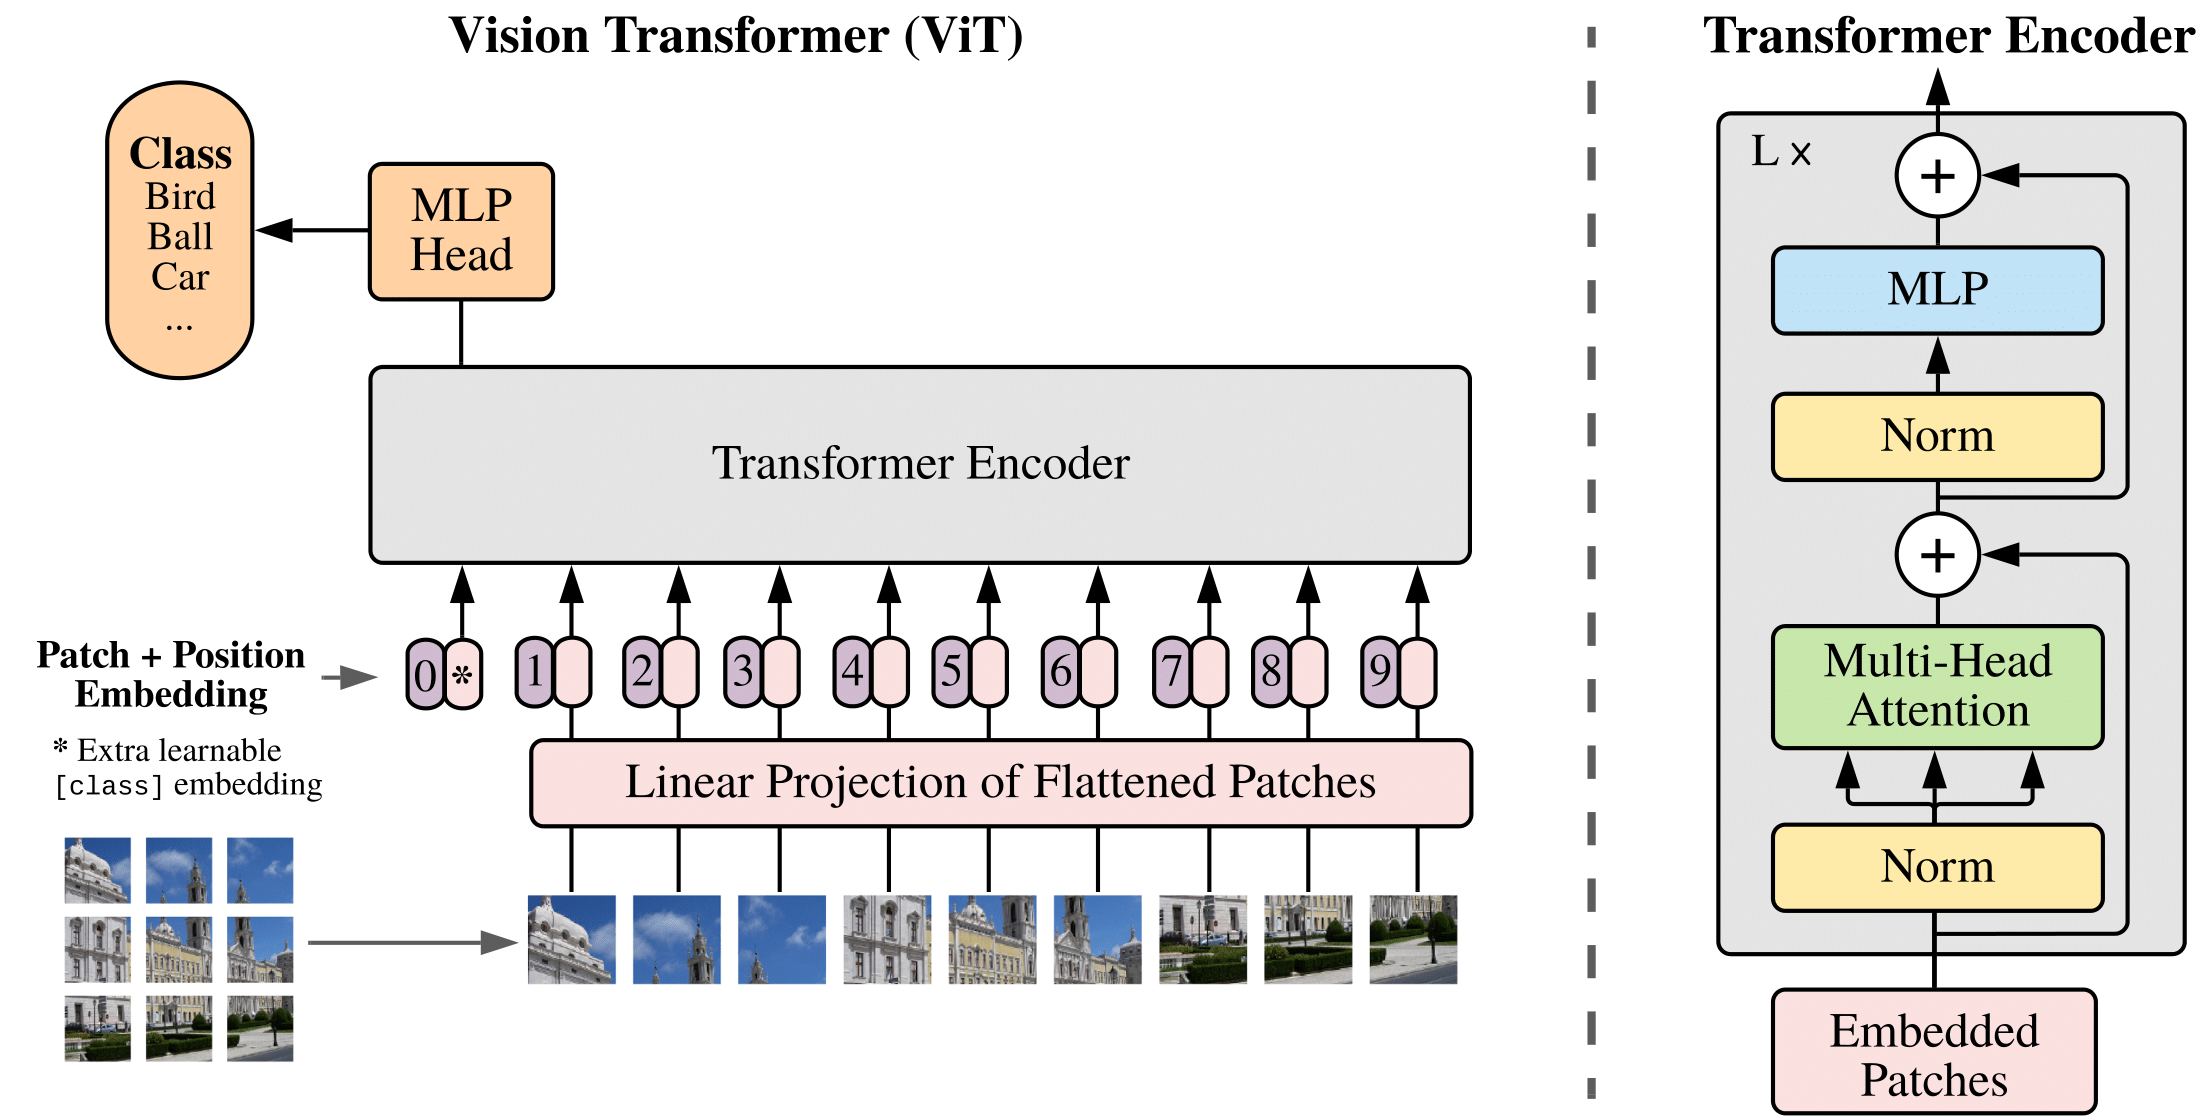
\includegraphics[width=0.7\linewidth]{modeling/visionTransformer.png}  
\caption{Vision Transformer (ViT) architecture \citep{ViT}.}
\label{modeling.visionTransformer}
\end{figure*}

The image encoder of CLIP uses Vision Transformer (ViT) introduced in \cite{ViT}. The architecture of ViT is very similar to the original transformer introduced in \cite{attentionAllYouNeed}. 
In order to reuse the transformer model, ViT needs to first turn an image of size $H\times W \times C$, ($H$, $W$, $C$ stands for image height, width, channel size, respectively), into a sequence of ``tokens'', similar to the text input.  
To do so, \cite{ViT} reshapes the image to size $N \times (P^2 \cdot C)$, where $N$ is the number of patches and $P$ the patch size; the reshaped image can be seen as a sequence of $N$ image tokens, each having a dimension of $P^2 \cdot C$. Each image token is then passed through a linear layer to be mapped to dimension $D$, similar to the model dimension $d_{model}$ earlier. 
In the version of CLIP that we used, $H = W = 224$, $C = 3$, $P = 32$, and $D = 768$. 
As explained in \cite{ViT}, before passing into the transformer, we also need to prepend a \texttt{[class]} token at the front the sequence, whose embedding at the last layer of the transformer will be used as the representation for the entire image. In this way, each image is represented as a sequence of $7\times 7 + 1 = 50$ tokens, illustrated as purple boxes in Figure \ref{modeling.visionTransformer}. The pink boxes that are right next to the patch embeddings represent position embeddings, with a similar function to encoder sequence order information as in the text transformer. 
For the CLIP image encoder, layer normalization is applied to the input before passing into the transformer and to the output at the last layer.



\subsection{Pre-Training with Contrastive Objective and Natural Language Supervision} \label{clip.objective}
learning an open set of visual concepts from natural language natural language supervision compared to standard crowd-sourced labeling for image classification

\begin{figure*}[!htb]
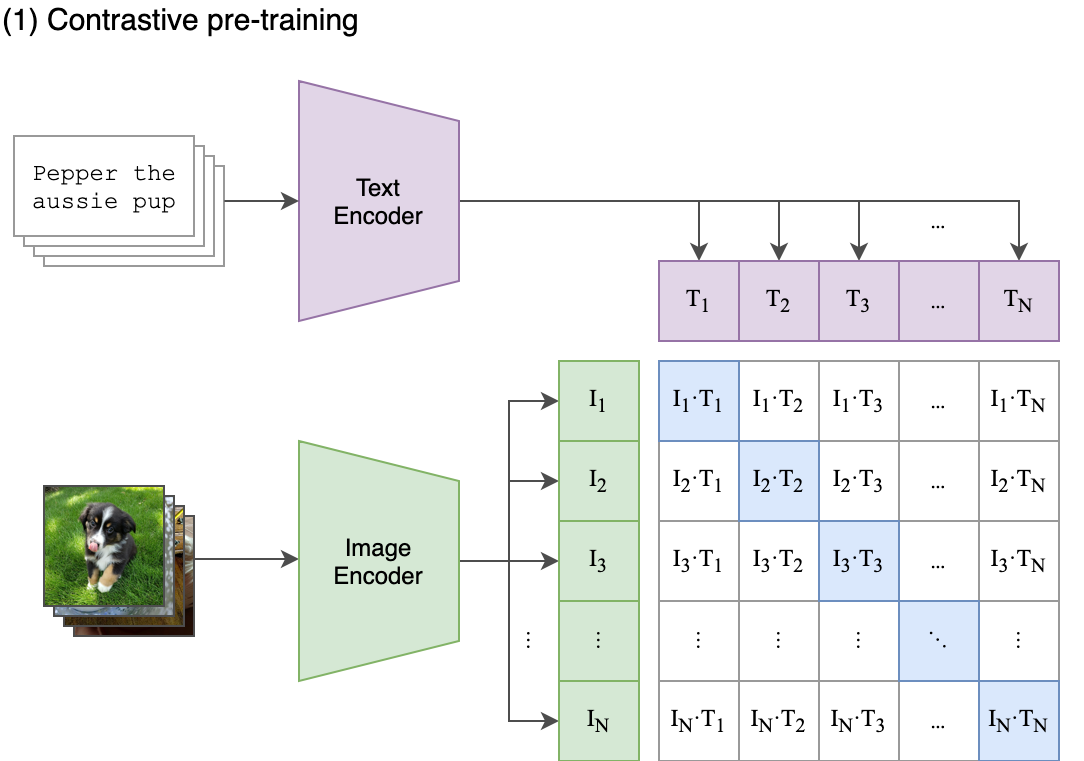
\includegraphics[width=0.7\linewidth]{modeling/CLIP.png}  
\caption{CLIP uses contrastive pre-training instead of generative objective to learn joint vision-language embeddings. This image is taken from Figure 1 in the original CLIP paper \citep{CLIPpaper}.}
\label{modeling.clip.pretrainingobj}
\end{figure*}

It is difficult to predict the exact captions for an image, since there is usually a wide variety of text descriptions co-occuring with images, so instead CLIP turns to contrastive objectives and solves the problem of determining which text and image should be matched together. 
As shown in Figure \ref{modeling.clip.pretrainingobj}, during pre-training, for a batch of $N$ (text,image) pairs, CLIP obtains $N$ image features and $N$ text features from the encoders. It then calculates the cosine similarities between each of the $N \times N$ pairings of the image and text features. The values are used as logit scores for calculating symmetric cross-entropy loss used to train the network.      


CLIP is trained on 400 million (image, text) pairs collected form a variety of publicly available sources on the Internet.

The query list that is used to compile these (image,text) pairs is the union of (1) words that occur $\geq 100$ times in English Wikipedia; (2) names of Wikipedia articles whose search volume is above certain threshold; (2) high pointwise mutual information (PMI) bi-grams, and (4) $117,000$ WordNet synsets, or sets of cognitive synonyms. 

\subsection{Image Pre-Processing}
We use the data provided by SPG \citep{spg_paper}, which provides JSON files of the Quick,Draw! sketches in vector format: each sketch is composed of a sequence of $n$ strokes $S_i, i \in [n]$, and $S_i$ is a sequence of vectors $(\delta x,\delta y, p, l)$. $\delta x$ and $\delta y$ are changes in the $x,y$ coordinates with respect to the previous point; for the first point, it is with respect to $(25,25)$. All points are assumed to be drawn on a $256 \times 256$ canvas. $p=1$ if the point is the last point in the current stroke, and $p=0$ otherwise. The SPG dataset provides annotation for semantic segmentation of the sketches, so $l$ is a number representing the semantically meaningful object part.  

% We obtained the rendered sketches by using \texttt{Pycairo}, which is a Python module providing bindings for the cairo graphics library. We use a line width of $5$. After rendering, we manually examined the sketches and filter out face sketches that do not have a pair of eyes, a mouth and the face outline; we also filter out angel sketches that are incomplete or have all the parts merged together, possibly due to collection errors in SPG.   

\subsection{Text Pre-Processing}
We used the \texttt{spacy} package to preprocess the text. \texttt{spacy} provides trained natural language processing pipeline and includes models for, for example, token-to-vector and part-of-speech tagging. We use the \texttt{en\_core\_web\_sm} pipeline and its lemmatizer to reduce words to their basic forms. Moreover, we lower-case all words and remove punctuation, a list of which is provided by \texttt{Python} \texttt{string} package, \texttt{string.punctuation}. We also remove words like \textit{shaped}, \textit{sized}, \textit{and}, \textit{like}, since they act like stop words and do not provide additional visual descriptions of the sketches. Text descriptions are also tokenized by CLIP's tokenizer before passing into CLIP text encoder.     

\section{Loss Function}
During training, for a given batch size $N$, we have $N$ sketch-text pairs, $(s_k,t_k), k\in [N]$. 
As explained in \cite{CLIPpaper}, we can treat each batch as containing $N$ visual concepts expressed through language.    
To pre-train/fine-tune CLIP, we perform \textit{classification} over these $N$ visual concepts, using cross-entropy loss on the dot-product of the (image,text) embeddings. 
Let $I_f \in \mathbb{R}^{N \times 512}$ be image embedding for the $N$ images in the batch outputted by the image encoder; similarly, 
let $T_f \in \mathbb{R}^{N \times 512}$ be text embedding for the $N$ captions in the batch outputted by the text encoder. 
We then use dot-product to generate.

\begin{equation}
\begin{split}
    \text{image encoder: } E_i \\
    \text{text encoder: } E_t \\
    I_1^{'},\dots, I_N^{'} \\
    T_1^{'},\dots, T_N^{'} \\
    I_1,\dots, I_N \\
    T_1,\dots, T_N \\
\end{split}
\end{equation}


By calculating pairwise dot-product $I_i \cdot T_j$, we obtain a logit matrix $X$ of dimension $N\times N$, where $X_{ij} = I_i \cdot T_j$. Through softmax, if we normalize each row, then we obtain a distribution over the texts of how likely the $i$-th image is paired with the $j$-th caption; similarly, normalizing each column via softmax, we obtain a distribution over the images of how likely the $j$-th caption is paired with the $i$-th image.   
% image logits $X_v$ over the text descriptions and text logits $X_t$ over the images. 
The ground-truth $Y$ is pairing the $i$-th image with the $i$-th caption.  
$Y = \begin{bmatrix}1 & 2 & \cdots & N \end{bmatrix}^T $ 
To calculate the loss $L_I(X, Y)$ of selecting the correct caption for each image:
\begin{equation}
\begin{split}
    L_I(X, Y) = \dfrac{1}{N} \sum_{i=1}^N -\log\frac{\exp\{ {X}_{i,i} \}}{ \sum_{j=1}^N \exp\{ {X}_{i,j} \} }
\end{split}
\end{equation}

To calculate the loss $L_T(X, Y)$ of selecting the correct image for each caption:
\begin{equation}
\begin{split}
    L_T(X, Y) = \dfrac{1}{N} \sum_{j=1}^N -\log\frac{\exp\{ {X}_{j,j} \}}{ \sum_{i=1}^N \exp\{ {X}_{i,j} \} }
\end{split}
\end{equation}


The final loss is defined as:
$$L = \dfrac{1}{2} (L_I(X, Y) + L_T(X, Y))$$

\section{Data Augmentation}
As mentioned above, our dataset has a small number of sketches: 572 face sketches and 787 angel sketches.  



% Text representation. 
% We have RNN to model the sequence of strokes. Can we still use RNN to model the sequence of words? Does the length of the sentence matter? If we only have adjectives, how can we effectively model these words? 
% What are methods that can model the semantics of these words alone? 
% Where can we find existing representations of these words? How are traditional text-image synthesis methods modeling the words? 
% Reed et al. [28] obtain the text encoding of a textual description by using a pre-trained character-level convolutional recurrent neural network (char-CNN-RNN). The char-CNN-RNN is pretrained to learn a correspondence function between text and image based on the class labels. 